\section{Architecture}
\begin{frame}{Architecture}

\begin{itemize}

    \item PlanetRenderer 
        \begin{itemize}
            \item Projet déjà existant
            \item https://github.com/Illation/PlanetRenderer (Robert Lindner)\\
    \end{itemize}

    \item Création des cartes de hauteurs
    \begin{itemize}
        \item Gestion des entrées utilisateur
        \item Différents bruits
        \begin{itemize}
            \item simplex
            \item perlin
            \item ...
        \end{itemize}
    \end{itemize}

\begin{figure}
%    \begin{flushright}
   
\includegraphics[scale=0.40]{img/nosie.png}
   \caption{Exemple de bruit src: \url{https://github.com/simongeilfus/SimplexNoise}}
%   \end{flushright}
\end{figure}

    
%    \item Statistique
%    \begin{itemize}
%        \item 27 classes
%        \item $\sim$4300 lignes de codes
%    \end{itemize}
\end{itemize}

\end{frame}


% ----------
% SCREENSHOT

% FBM 1024*1024

\begin{frame}
  \begin{figure}[!ht]
    \centering
    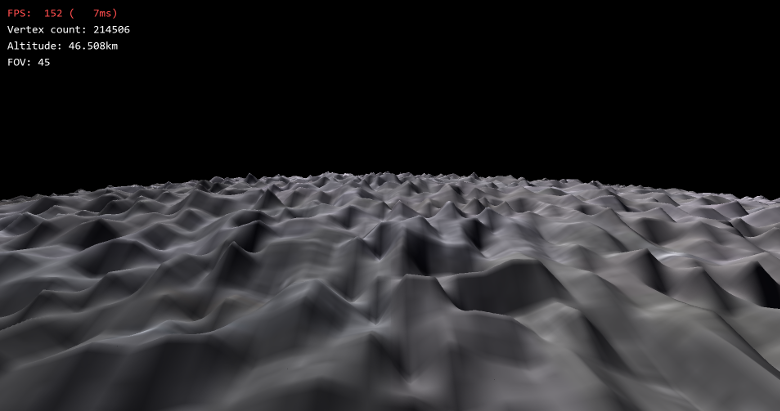
\includegraphics[width=10cm]{img/landscape.png}
    \caption{Planète procédurale FBM}
    \label{fig:landscape}
  \end{figure}
\end{frame} 

\begin{frame}{Architecture}

Scène
\begin{itemize}
    \item Initialise Caméra, Time
    \item Créer la planète
\end{itemize}

\begin{figure}
   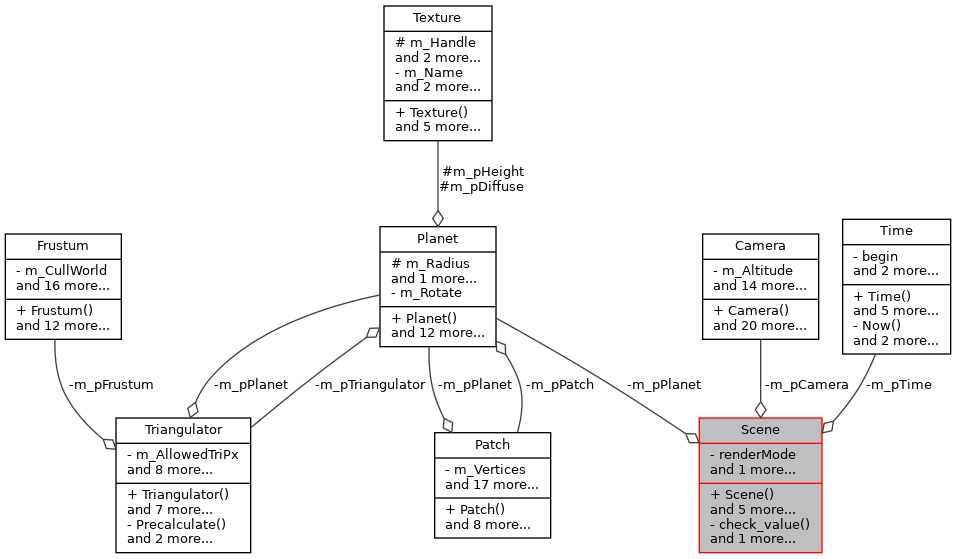
\includegraphics[scale=0.30]{img/scene_uml.png}
   \caption{Diagramme de classe}
\end{figure}

\end{frame}

\begin{frame}{Architecture}

Planète
\begin{itemize}
    \item Génère la carte de hauteur
    \item Créer la planète
    \item Classe Triangulator, Patch
\end{itemize}

\begin{figure}
   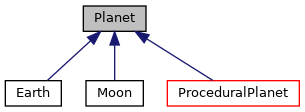
\includegraphics[scale=0.40]{img/planet_inh.png}
   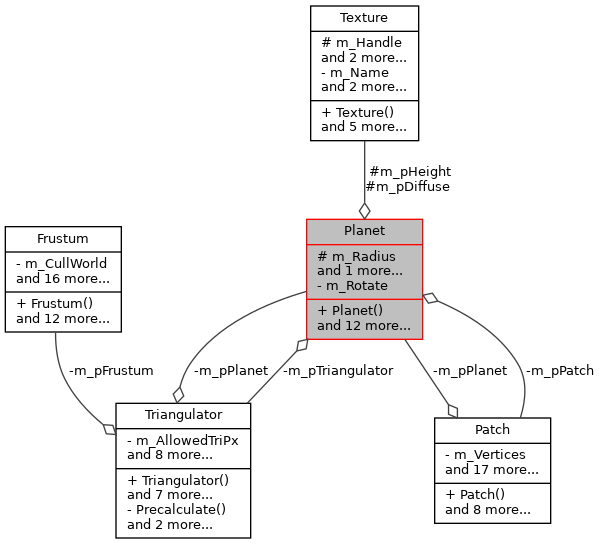
\includegraphics[scale=0.30]{img/planet_uml.png}
   \caption{Classe Planète}
\end{figure}

\end{frame}

\begin{frame}{Architecture}

\begin{itemize}
    \item Classe Triangulator : Génére la géométrie de la planète
    \begin{itemize}
        \item Classe Frustum : Représente le cône de vision    
    \end{itemize}
    \item Classe Patch : Gère le morphing
    \item Classe ArgvParser: Gère les entrées utilisateurs
\end{itemize}
\end{frame}


